\section{Muon Trigger Overview}

Each of the three muon detector systems in CMS participates in the Level-1 muon trigger for
coverage and redundancy. For the DT and CSC systems ($|\eta|$ $<$ 1.2 and $|\eta|$ $>$ 0.9, respectively),
the front-end trigger primitive generator (TPG) electronics identify track segments from the hit
information registered in multiple gas planes of a single measurement station. These segments
are collected and then transmitted via optical fibres to regional Track-Finders in the electronics
service cavern, which then apply pattern recognition algorithms in order to identify muon
candidates and measure their momenta from the magnetic bending in the return yoke between
several measurement stations. Information is shared between the DT Track-Finder (DTTF)
and CSC Track-Finder (CSCTF) for efficient coverage in the region of overlap between the two
systems at $|\eta|$ $\approx$ 1. The hits from the RPC system ($|\eta|$ $<$ 1.6) are directly sent from the front-
end electronics to PAttern Comparator (PAC) logic boards that identify muon candidates.

\begin{figure}[tbh]
	\begin{center}
		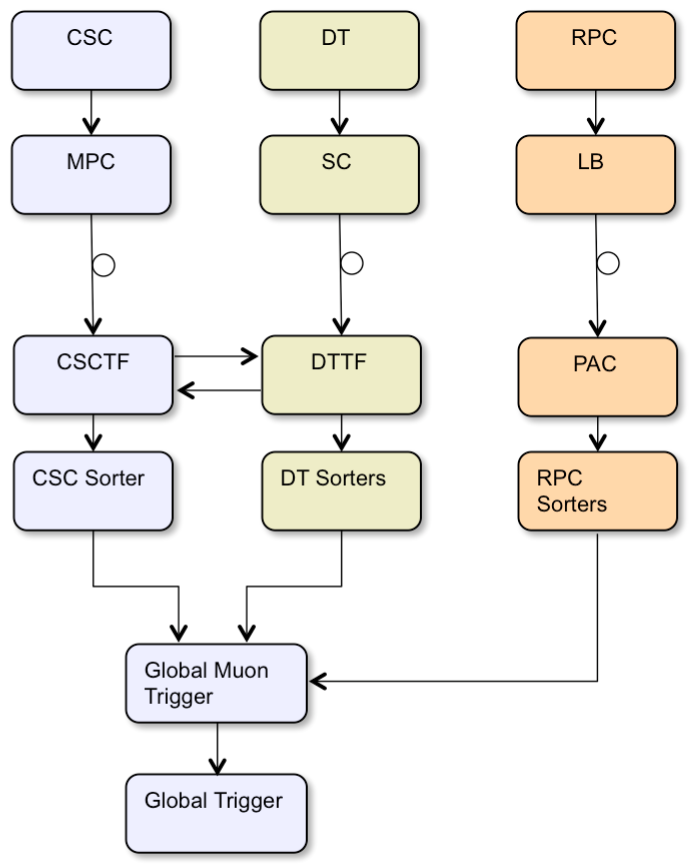
\includegraphics[width=0.48\linewidth]{figures/dataflow_current_L1_trigger.png}
	\end{center}
	\caption{Data-flow of the present L1 muon trigger. \label{fig:l1_muon_trig} }
\end{figure}

The three regional track-finders sort the identified muon candidates and transmit to the Global
Muon Trigger (GMT) up to 4 (CSCTF, DTTF) or 8 (RPC) candidates every bunch crossing. Each
candidate has been assigned a pT and quality code as well as $\eta$ and $\phi$ positions in the muon
system (with a granularity of $\approx$ 0.05). The GMT then merges muon candidates found by more
than one system to eliminate fake multi-muon triggers (with several options on how to select
pT between the candidates), and can suppress muon candidates in some regions of the detector
if their quality is low and they are unconfirmed by another muon system.